\section{Illuminance calculation}
Illuminance $E$ of a planar surface is the areal density of luminous flux incident on the surface \cite{Habel}:

\begin{equation}
E=\frac{d\Phi_{i}}{dA}
\end{equation}

Where:
\begin{description}
	\item[$d\Phi_{i}$] is the luminous flux incident on a surface
	\item[$dA$] is the surface area
\end{description}

Luminous intensity $I$ is the amount of luminous flux contained in a given solid angle. For a direction defined by angle $\gamma$ is luminous intensity of this angle defined as follows \cite{Habel}:

\begin{equation}
I_{\gamma}=\frac{d\Phi}{d\Omega}
\end{equation}

Where:
\begin{description}
	\item[$d\Phi$] is the amount of luminous flux contained in the solid angle $d\Omega$
	\item[$d\Omega$] is the solid angle with its axis pointing in direction~$\gamma$
\end{description}

As mentioned in section~\ref{sec:Road_Lighting_Design}, illuminances need to be calculated. Photometric properties of luminaires are defined in eulumdat files, containing luminous intensity distribution curves needed to obtain illuminances.

\begin{figure}[htb]
  \centering
  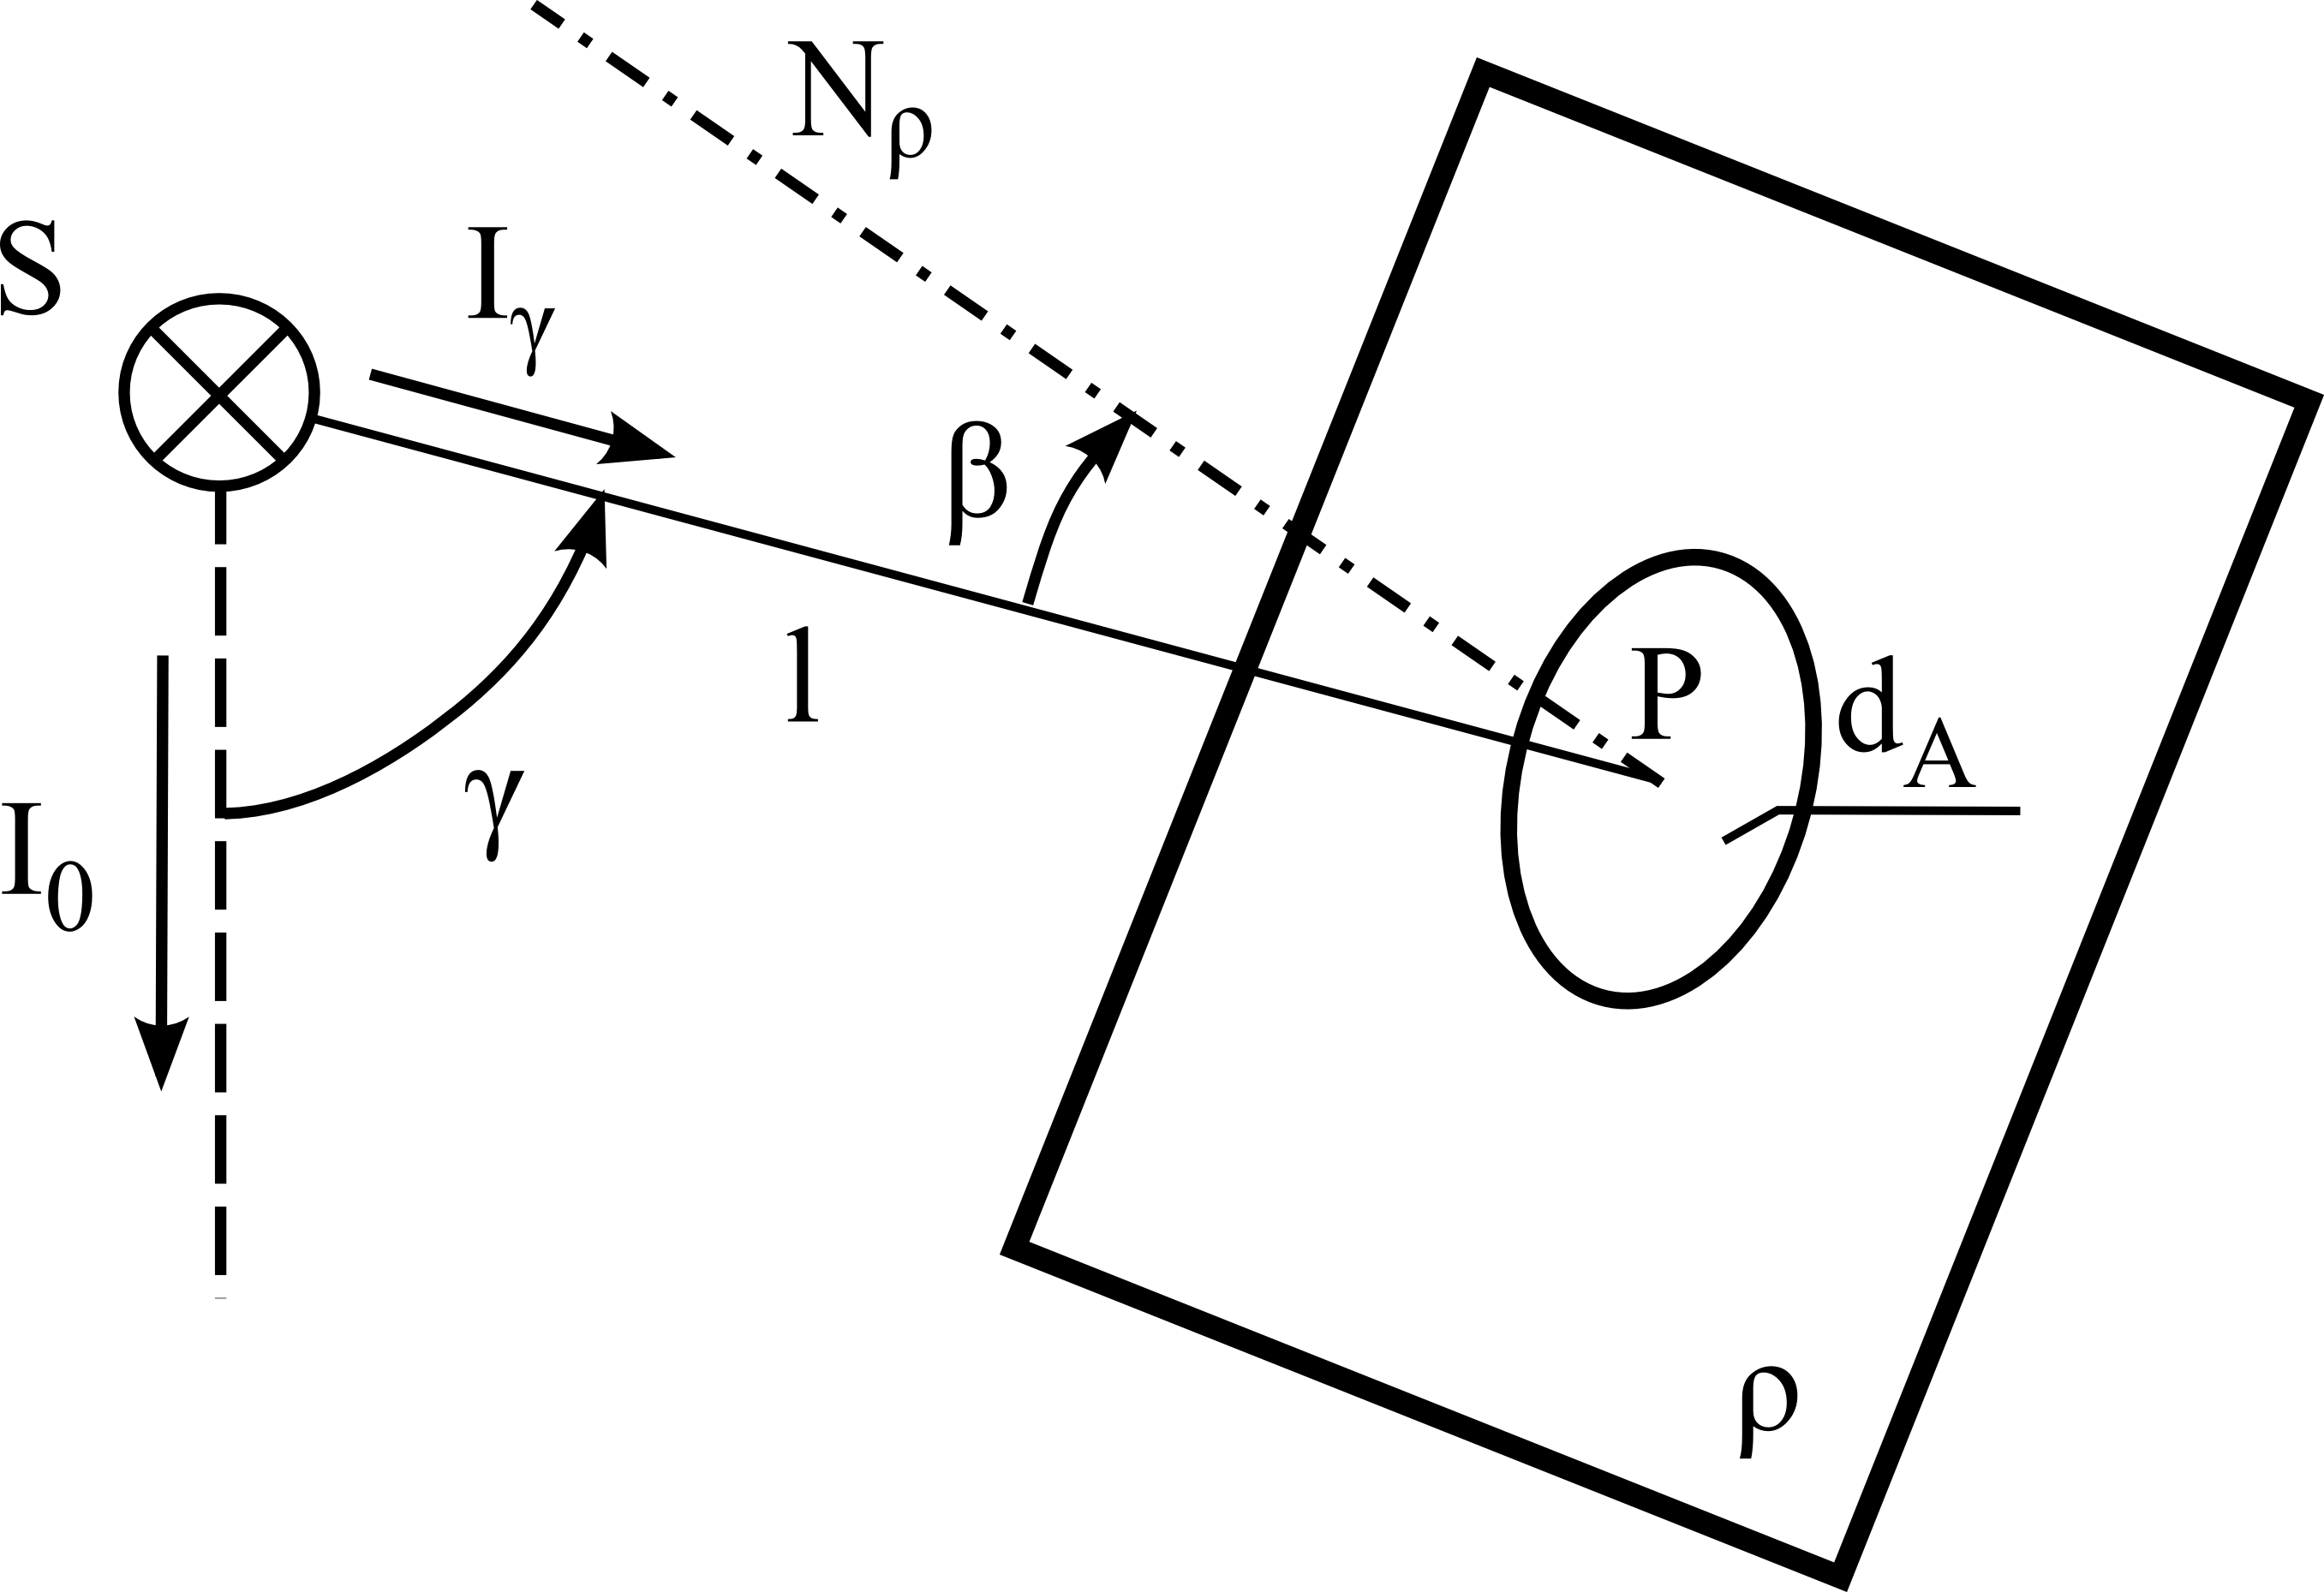
\includegraphics[width=0.8\columnwidth]{315_osvetlenost_bodovym_zdrojem}
  \caption{Facet $\rho$ illuminated with light source $S$}
  \label{fig:illuminance}
\end{figure}

According to~\cite{Habel} illuminance at point $P$ (as seen in figure~\ref{fig:illuminance}) illuminated by light source $S$ can be obtained by the following equation:

\begin{equation}
E_{P\rho}=\frac{I_{\gamma} \cdot cos \beta}{l^2}
\end{equation}

Where:
\begin{description}
	\item[$I_{\gamma}$] is the luminous intensity in the given direction $\gamma$
	\item[$\beta$] is the angle between the surface's normal $N_{\rho}$ and the $SP$ point join $l$
	\item[$l$] is the distance between the light source S and the point P of facet $dA$ of surface $\rho$
\end{description}

